
% This LaTeX was auto-generated from an M-file by MATLAB.
% To make changes, update the M-file and republish this document.

\documentclass{article}
\usepackage{graphicx}
\usepackage{color}

\sloppy
\definecolor{lightgray}{gray}{0.5}
\setlength{\parindent}{0pt}

\begin{document}

    
    
\subsection*{Contents}

\begin{itemize}
\setlength{\itemsep}{-1ex}
   \item Ejercicio 4 - Análisis estadístico de datos - ICA
   \item 1
   \item fastica.m
   \item 2
   \item Mezclas de las dos fuentes
   \item Blanqueo de las mezclas mediante PCA
   \item Separación con FastICA
   \item Estimando P y D
\end{itemize}


\subsection*{Ejercicio 4 - Análisis estadístico de datos - ICA}

\begin{verbatim}
clc; close all; clear all;
\end{verbatim}


\subsection*{1}

\begin{par}
Implemente el algoritmo de FastICA con aprendizaje deflacionario.
\end{par} \vspace{1em}
\begin{par}
Debajo se copia el código fuente de la función implementada. La descripción de la misma se encuentra dentro del código.
\end{par} \vspace{1em}


\subsection*{fastica.m}

\begin{verbatim}
dbtype fastica.m
\end{verbatim}

        \color{lightgray} \begin{verbatim}
1     function [sepMat] = fastica( X )
2     %[sepMat] = fastica( X ) devuelve la matriz de separación sepMat
3     %   Los versores de la descomposición se ubican como columnas en la matriz
4     %   de separación.
5     %   Las mezclas X deben ser de tamaño N x M, donde N corresponde a la
6     %   cantidad de mezclas y M a la cantidad de muestras que tiene cada señal.
7     %   Las mezclas en X deben tener media cero y la matriz de covarianza debe
8     %   ser identidad (realizar whitening de ser necesario)
9     
10    tolerancia = 1e-6; 
11    optimizando = 0;  %
12    [N, M] = size(X); % N-dimensiones, M muestras
13    
14    for p = 1:N
15        error = 1;    % inicia el ciclo de optimización
16        colineal = 0; % inicia el ciclo de optimización
17        w(:,p) = 2*rand(N,1)-1; % inicialización aleatoria de wp
18        
19        while (error > tolerancia) && ~colineal
20            want = w(:,p);
21            
22            % G(y) = (1/a) * log cosh (ay)
23            % g(y) = tanh(ay)
24            % gprima(y) = a(1-tanh(ay)^2)
25            a = 1;
26            g = ones(N,1) * tanh(a * want' * X) ;% g es de tamaño N x M
27                                                 % ones genera N filas iguales
28                                                 % de g evaluada en cada
29                                                 % a*want'*x
30            gprima = a * (1 - tanh(a * want' * X).^2); % gprima es de tamaño 1 x M
31            
32            % Expresion para cada muestra
33            % wnuevo = E[g(w'*x)*x] - E[gprima(w'*x)]*w
34            % Expresion usando el vector X de todas las muestras
35            w(:,p) = (-1) *(mean(g .* X, 2) - mean(gprima) * want);
36                 
37            % El valor esperado de la ecuación original es estimado por el 
38            % valor medio
39            % g .* X es el equivalente de g(w'*x)*x considerando todos los
40            % ejemplos
41            
42            % se ortogonaliza respecto a las wp ya encontradas
43            for j = 1:p-1
44                w(:,p) = w(:,p) - (w(:,p)' * w(:,j)) * w(:,j);
45            end
46            
47            % se normaliza wp
48            w(:,p) = w(:,p) ./ norm(w(:,p));
49            
50            error = norm(w(:,p) - want); % chequea convergencia de w(:,p)
51            colineal = (1-abs(dot(want,w(:,p)))) < tolerancia; % si es colineal
52                                                               % finalizo la
53                                                               % búsqueda
54        end
55    end
56    
57    sepMat = w; % encontrados todos los wp los paso a la salida de la función
58    
59    end
60    

\end{verbatim} \color{black}
    

\subsection*{2}

\begin{par}
A partir de datos de dos mezclas, obtenidos mediante dos fuentes laplacianas y una matriz de mezcla aleatoria, utilice FastICA para lo siguiente:
\end{par} \vspace{1em}
\begin{enumerate}
\setlength{\itemsep}{-1ex}
   \item Para cada etapa (fuentes, mezclas, señales blanqueadas, señales   separadas) dibuje un gráfico de dispersión de las variables.
   \item Pruebe con fuentes con distribución gaussiana y laplaciana, para
   \item Luego de la separación, estime las matrices $\mathbf{P}$ y $\mathbf{D}$   obtenga la matriz $\mathbf{W}$ correspondiente.
\end{enumerate}
\begin{verbatim}
N = 1000; % Cantidad de muestras

% Fuentes laplacianas
s{1} = randlap(N, 2 , 2)';
s{2} = randlap(N, -5,0.4)';

% Se corroboran los signos para impedir que las mezclas sean iguales
signos = ones(2);
while isequal(signos(1,:),signos(2,:)) || isequal(signos(1,:), -signos(2,:))
    signos = sign(rand(2)-0.5);
end
% Generacacion de la matriz de mezcla
A = (2*rand(2)-1) .* signos;  % Mezcla no ortogonal
% A = [0.6 0.8; 0.5 -0.2];

% suptit{1} = 'Fuentes laplacianas';
\end{verbatim}


\subsection*{Mezclas de las dos fuentes}

\begin{verbatim}
X = mezclar(A,s{1},s{2});
\end{verbatim}


\subsection*{Blanqueo de las mezclas mediante PCA}

\begin{verbatim}
[E, lambdas] = mipca(X);
% E: matriz cuyas columnas son los versores de las direcciones
%    principales.
% lambdas: es un vector con los autovalores

Dmenos1medio = diag(sqrt(lambdas.^(-1)));% matriz con las inversas de los
                                         % lambdas en la diagonal principal

Xmean = repmat(mean(X,2), 1, size(X,2)); % media de las mezclas

Z = Dmenos1medio * E'  * (X - Xmean);    % señales blanqueadas
\end{verbatim}


\subsection*{Separación con FastICA}

\begin{verbatim}
W = fastica(Z); % me devuelve la matriz de separación

Y = W' * Z; % Separación de las fuentes mediante la matriz dada por fastica
\end{verbatim}


\subsection*{Estimando P y D}

\begin{par}
Como se cumple que $\mathbf{y} = \mathbf{W}^T\mathbf{x} = \mathbf{W}^T\mathbf{A}\mathbf{s}$, es posible fijarse cual de las dos fuentes aporta mas a cada señal recuperada y asi poder determinar si están permutadas las señales recuperadas con las fuentes.
\end{par} \vspace{1em}
\begin{par}
Así, en primer lugar busco la matriz $\mathbf{P}$ que cumpla $\mathbf{P} \mathbf{D} = \mathbf{W}^T\mathbf{A}$. Hay solo dos posibilidades para esta matriz, la identidad, o un matriz con sólo unos en la diagonal secundaria. Para esto me fijo en cada renglon de la matriz $\mathbf{W}^T\mathbf{A}$ y defino una matriz $\mathbf{P}$ a partir de los máximos componentes por renglón.
\end{par} \vspace{1em}
\begin{verbatim}
WA = W' * A;
[~, maxwa] = max(abs(WA),[],2);

P = zeros(2);
P(1,maxwa(1)) = 1;
P(2,maxwa(2)) = 1;
\end{verbatim}
\begin{par}
La anterior forma de encontrar $\mathbf{P}$ no está funcionando como se esperaba por lo que para decidir la permutación realizo una comparación entre las señales recuperadas y las fuentes.
\end{par} \vspace{1em}
\begin{verbatim}
s1y1 = dot(s{1}-mean(s{1},2),Y(1,:)) ./ size(Y,2); % fuente 1 vs recup 1
s1y2 = dot(s{1}-mean(s{2},2),Y(2,:)) ./ size(Y,2); % fuente 1 vs recup 2
s2y1 = dot(s{2}-mean(s{1},2),Y(1,:)) ./ size(Y,2); % fuente 2 vs recup 1
s2y2 = dot(s{2}-mean(s{2},2),Y(2,:)) ./ size(Y,2); % fuente 2 vs recup 2

auxs1 = [s1y1, s1y2]; % el maximo me dice cual corresponde a fuente 1
auxs2 = [s2y1, s2y2]; % el maximo me dice cual corresponde a fuente 2
[~, s1max] = max(abs(auxs1));
[~, s2max] = max(abs(auxs2));

P = zeros(2) ;
P(1,s1max) = 1; % asigno los 1 de acuerdo a lo encontrado
P(2,s2max) = 1; % asigno los 1 de acuerdo a lo encontrado

% como P y su inversa son iguales calculo D = Pinv * W' * A

D = P * WA;

fprintf(['P = [%0.2f %0.2f],\t D = [%0.2f %0.2f]\n'...
         '    [%0.2f %0.2f],\t     [%0.2f %0.2f]\n\n'],...
          P(1,:), WA(1,:), P(2,:), WA(2,:) );


% Graficando cada etapa
subplot(2,2,1)
scatter(s{1}, s{2}); axis equal;
title({'Fuentes'})
xlabel('s_1'); ylabel('s_2');

subplot(2,2,2)
scatter(X(1,:), X(2,:)); axis equal;
title({'Mezclas'})
xlabel('x_1'); ylabel('x_2');

subplot(2,2,3)
scatter(Z(1,:), Z(2,:)); axis equal;
title({'Señales blanqueadas'})
xlabel('z_1'); ylabel('z_2');

subplot(2,2,4)
scatter(Y(1,:), Y(2,:)); axis equal;
title({'Señales separadas'})
xlabel('y_1'); ylabel('y_2');
\end{verbatim}

        \color{lightgray} \begin{verbatim}P = [0.00 1.00],	 D = [0.85 -0.14]
    [1.00 0.00],	     [-0.44 -0.35]

\end{verbatim} \color{black}
    
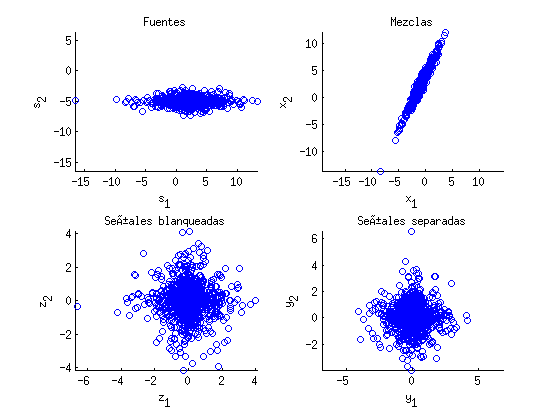
\includegraphics [width=4in]{Ejercicio4_01.png}
\begin{par}
En las gráficas se muestra cada una de las etapas requeridas.
\end{par} \vspace{1em}
\begin{verbatim}
% Comparación entre señales separadas y fuentes
figure
subplot(2,2,1)
plot(s{1}(1:60)); ylim([-10, 10]);
ylabel('s_1')

subplot(2,2,2)
plot(s{2}(1:60)); ylim([-10, 10]);
ylabel('s_2');

subplot(2,2,3)
plot(Y(1,1:60)); ylim([-10, 10]);
ylabel('y_1');

subplot(2,2,4)
plot(Y(2,1:60)); ylim([-10, 10]);
ylabel('y_2');
\end{verbatim}

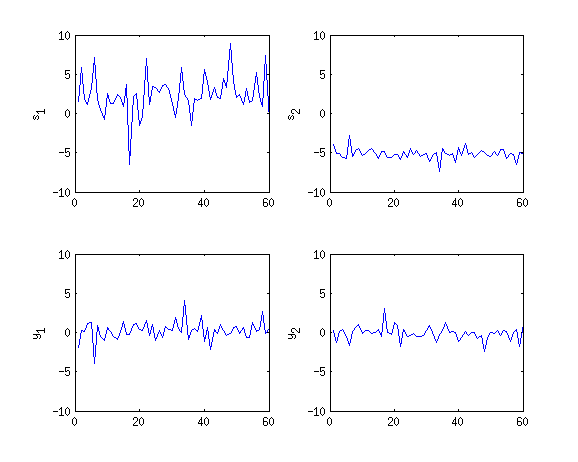
\includegraphics [width=4in]{Ejercicio4_02.png}
\begin{enumerate}
\setlength{\itemsep}{-1ex}
   \item ¿La matriz de separación $\mathbf{W}$ es la inversa de la matriz de mezcla $\mathbf{A}$ utilizada?
\end{enumerate}
\begin{par}
No lo es, en el caso ideal lo sería. En la práctica se espera obtener $\mathbf{P} \mathbf{D} = \mathbf{W}^T\mathbf{A}$, donde $\mathbf{P}$ es una matriz de permutación y \ensuremath{\backslash}mathbf\{D\} es una matriz de escalado (también involucra el signo para invertir la señal de ser necesario).
\end{par} \vspace{1em}
\begin{enumerate}
\setlength{\itemsep}{-1ex}
   \item ¿Cómo se afecta este resultado si agrega una componente de ruido gaussiano al modelo generativo?
\end{enumerate}
\begin{par}
La base del funcionamiento de ICA está en maximizar la lejanía de las distribuciones de cada señal recuperada de la distribución gaussiana. Si el ruido gaussiano tiene una potencia importante en relación a las fuentes es de esperar que no se logren recuperar. Si el ruido no enmasacara por demás las fuentes es posible recuperar las fuentes.
\end{par} \vspace{1em}
\begin{enumerate}
\setlength{\itemsep}{-1ex}
   \item ¿Qué ocurre si una de las fuentes es gaussiana? ¿Y si ambas lo son?
\end{enumerate}
\begin{par}
Si una de las fuentes es gaussiana todavía es posible encontrar las fuentes, si las dos lo son no es posible.
\end{par} \vspace{1em}
\begin{verbatim}
% % % % % for ss = 1:2
% % % % %     figure
% % % % %     for aa = 1:2
% % % % %         X = mezclarconruido(A{aa},s{2*ss-1},s{2*ss}); % Mezclas
% % % % %
% % % % %         W = mipca(X); % Obtengo la Matriz de Proyección de X sobre las
% % % % %                       % componentes principales
% % % % %
% % % % %         Y = W * X; % Proyecto los datos sobre las direcciones principales
% % % % %
% % % % %         subplot(2,3,1+3*(aa-1))
% % % % %         scatter(s{2*ss-1}, s{2*ss}); axis equal;
% % % % %         title({'Fuentes';['columnas ' titort{aa}]} )
% % % % %         xlabel('s_1'); ylabel('s_2');
% % % % %
% % % % %         subplot(2,3,2+3*(aa-1))
% % % % %         scatter(X(1,:), X(2,:)); axis equal;
% % % % %         hold on;
% % % % %         x1m = mean(X(1,:));
% % % % %         x2m = mean(X(2,:));
% % % % %         plot(x1m + [0 5*W(1,1)],x2m + [0 5*W(1,2)], 'k','LineWidth',2)
% % % % %         plot(x1m + [0 5*W(2,1)],x2m + [0 5*W(2,2)], 'k','LineWidth',2)
% % % % %         hold off
% % % % %         title({'Mezclas';['columnas ' titort{aa}]} )
% % % % %         xlabel('x_1'); ylabel('x_2');
% % % % %
% % % % %         subplot(2,3,3+3*(aa-1))
% % % % %         scatter(Y(1,:), Y(2,:)); axis equal;
% % % % %         title({'Señales separadas';['columnas ' titort{aa}]} )
% % % % %         xlabel('y_1'); ylabel('y_2');
% % % % %
% % % % %         A{aa}
% % % % %         inv(A{aa})
% % % % %         W
% % % % %     end
% % % % %     suptitle(suptit{ss})
% % % % % end

% % % % % % % % % % Xmean(:,1)
% % % % % % % % %
% % % % % % % % %
% % % % % % % % % D = zeros(2);
% % % % % % % % % D(1,1) = auxs1(s1max);
% % % % % % % % % D(2,2) = auxs2(s2max);
% % % % % % % % % D;
% % % % % % % %
% % % % % % % % % Y = Y + W' *  Xmean;
% % % % %
% % % % % Srecup = inv(P * D) * Y;
% % % % %
% % % % %
% % % % % subplot(3,2,5)
% % % % % plot(Srecup(1,1:60)); ylim([-10, 10]);
% % % % % ylabel('s.recup_1');
% % % % %
% % % % % subplot(3,2,6)
% % % % % plot(Srecup(2,1:60)); ylim([-10, 10]);
% % % % % ylabel('s.recup_2');
\end{verbatim}



\end{document}
    
